% Especificaciones del tamaño de letra, tamaño de hoja, márgenes, librerias, etc.
\documentclass[12pt, letterpaper]{article}
\usepackage[english]{babel}
\usepackage[utf8]{inputenc}
\usepackage[T1]{fontenc}
\usepackage{amsmath}
\usepackage{graphicx}
\usepackage{subcaption}
\usepackage{hyperref}
\usepackage{url}
\usepackage{amssymb}
\usepackage{float}
\usepackage[margin=1in]{geometry}
\renewcommand{\baselinestretch}{1.5}

% Enlace Bibliografía
\usepackage{csquotes}
\usepackage[notes,backend=biber]{biblatex-chicago}
\addbibresource{referencias.bib}

% Titulo, autores, fecha.
\title{Práctica \#4: Análisis Estático}
\author{Carlos Vásquez 1155057}

% Inicio del documento
\begin{document}
\maketitle
\section*{Introducción}

Anteriormente, en la práctica \#3, se analizó tensión de von mises que experimentaba una viga. Es posible calcular el esfuerzo unitario que se aproximará al análisis de tensión de von mises. Uno de los cálculos que es posible realizar es el de la deformación unitaria. En la práctica pasada fue omitido, sin embargo se analizarán en este reporte.

A diferencia de las prácticas anteriores, ahora trabajaremos en SOLIDWORKS, las diferencias entre SOLIDWORKS y CATIA no son muchas, realmente en lo que mayormente varían es en simples decisiones estéticas y en su GUI general, pero esto no los exime a ambos de el diseño paramétrico de piezas y análisis complejos.

El objeto que se analizó es un cilíndro de 3 cm de diámetro y 5 cm de altura.

\begin{figure}[H]
	\centering
	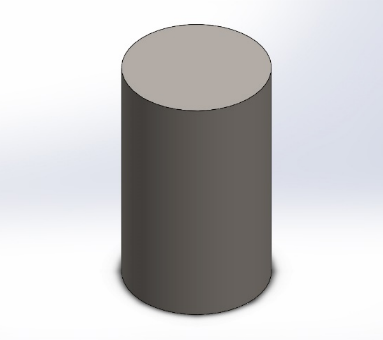
\includegraphics[width=0.4\textwidth]{cilinder.png}
	\caption{Modelo del objeto que se analizará.}
\end{figure}

\section*{Desarrollo}
Ya hemos observado el esfuerzo que se genera en un objeto sólido si a éste se le aplica una carga y lo hemos descrito matemáticamente como:

\begin{equation}
	\sigma = \frac{P}{A}
\end{equation}
Esto lo veremos más adelante para calcular el esfuerzo que experimentará nuestra pieza cilíndrica modelada. Es claro que en el cálculo se harán bastantes suposiciones e idealizaremos el modelo. Además de ésto también nos apoyaremos en el concepto de \textit{deformación unitaria}.

La deformación unitaria nos es útil para entender cómo un objeto se deforma ante distintas cargas. Dada la longitud original de un objeto \textit{L} y el elongamiento que ete objeto sufre al aplicarse una fuerza, $\delta$, la deformación unitaria puede ser expresada como la razón de la elongación sufrita y la longitud original del objeto en cuestión\autocite{MM}:

\begin{equation}
	\epsilon = \frac{\delta}{L}
\end{equation}

La razón por la cual utilizamos la deforación unitaria es sencilla. La deformación junto con un diagrama de carga-deformación nos dice las propiedades con las que cuenta un material, sin embargo no es posible emplearse directamente para predecir la deformación de una varilla del mismo material pero de diferentes dimensiones. Se observa que si se produce una deformación $\delta$ en una varilla BC por una carga \textbf{P}, se requiere una carga 2\textbf{P} para causar la misma deformación en una varilla B'C' de la misma longitud pero con una sección transversal de 2A. Es por este motivo que se utiliza la deformación unitaria. Cuando comparamos el esfuerzo en contraste a la deformación unitaria entonces obtenemos los diagramas \textit{esfuerzo-deformación}, los cuales nos dicen la propiedad de los materiales independientemente de sus dimensiones.

\section*{Cálculos}

Primero calcularemos el área del cilindro. Dado que nuestro cilindro tiene un diámetro de 3 cm, entonces su área será:
\begin{equation*}
\begin{split}
	A &= \pi(0.015\  m)^2 \\
	A &= 2.25 \times 10^{-4}\cdot \pi \ m^2
\end{split}
\end{equation*}

Para calcular el esfuerzo que experimentará el cilindro es sencillo dado que conocemos la carga aplicada a éste, la cual será de 100 kN a compresión:

\begin{equation}
	\begin{split}
	\sigma &= \frac{P}{A}\\
	\sigma &= \frac{100000\ N}{2.25 \times 10^{-4}\cdot \pi \ m^2}\\
	\sigma &\approx 141,471,060.5 Pa
	\end{split}
\end{equation}
Como observaremos más adelante en el reporte generado por SOLIDOWORKS, la tensión de von Mises promedio es aproximadamente 140,000,000 Pa, lo cual sugiere que el resultado es correcto y el análisis fue el adecuado.

Posterior al análisis del esfuerzo aplicado, también podemos calcular la deformación que sufrió el modelo. El material que se utilizó fue el ASTM A36 Acero y el reporte generado (que está anexado al final del documento) registra una deformación unitaria máxima de $7.802 \times 10^{-4}$, dado este dato, podemos calcular $\delta$:

\begin{equation}
	\begin{split}
		\epsilon = \frac{\delta}{L} \Longrightarrow \delta &= \epsilon L\\
		\delta &= (7.802 \times 10^{-4})(0.05\ m)\\
		\delta &\approx 3.901 \times 10^{-5} m\\
		\delta &\approx 0.03901\ mm
	\end{split}
\end{equation}


\section*{Conclusión}
Después de observar el análisis hecho por el software SOLIDWORKS y los cálculos realizados podemos concluir que son bastante parecidos y las variaciones son obvias dado que SOLIDWORKS utiliza aproximaciones mucho más cercanas a la realidad a través de las distintas propiedades del material utilizado. Es por este motivo que es capaz de arrojarnos una gráfica con los puntos en dónde la deformación y tensión son máximos, en lugar de realizar la suposición de que la fuerza que se aplica es distribuida uniformemente.

Gracias a este análisis es más fácil visualizar dónde se realizarán estos elongamientos y dónde sufre la mayor tensión nuestro modelo (que usualmente es de donde se ancla el modelo en cuestión).

A continuación se anexa el reporte generado con todos los datos del material utilizado y los resultados del análisis.
%%%%%  Bib
\renewcommand\refname{Referencias}
\printbibliography
\end{document}
